\documentclass{standalone}
\usepackage{tikz}
\usepackage{tikz-qtree}
\usepackage[makeroom]{cancel}
\usetikzlibrary{fit}

% ОПИСАНИЕ: деревья T0 и T1
\begin{document} 
	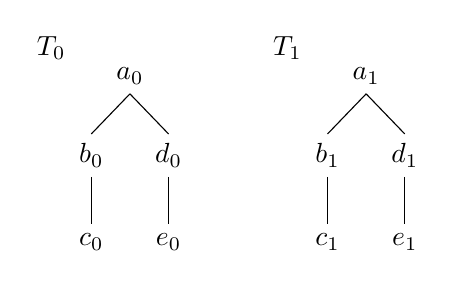
\begin{tikzpicture}[sibling distance=12pt]

	    \node (x) at (-1,0.4) {$T_0$} ;
	    \Tree [.$a_0$
	            [.$b_0$
	                $c_0$  ] 
	            [.$d_0$ 
	                $e_0$ ]]]
	    

	    \begin{scope}[xshift=3.0cm]
	    \node (y) at (-1,0.4) {$T_1$} ;
	    \Tree [.$a_1$
	            [.$b_1$
	                $c_1$  ] 
	            [.$d_1$ 
	                $e_1$ ]]]
	    \end{scope}

	\end{tikzpicture}
\end{document} 